\section{Experimental Validation}
\label{sec:experiments}

\subsection{Reconstruction Quality}
\label{sec:recon_quality}

Figure~\ref{fig:recon_grid} shows the best reconstruction per digit class on MNIST,
alongside the ×5-amplified residual map.  At ${\approx}40\,\text{dB}$ PSNR the
residuals are imperceptible; only slight blur on thin strokes remains.

\begin{figure}[htbp]
  \centering
  
\includegraphics[width=0.85\linewidth]{figures/fig_01_reconstruction_grid.png}
  \caption{%
    \textbf{Reconstruction quality per digit.}
    Each row shows the target image (left), the Gaussian splatting reconstruction
    (centre), and the absolute residual amplified by a factor of~5 (right, \emph{hot}
    colormap).
    Digits with thin strokes (1, 7) tend to achieve higher PSNR than complex, curved
    digits (8, 9) since thin strokes can be captured by fewer, elongated Gaussians.
    PSNR values are reported for the best encoding (lowest MSE) among the 5 images
    per digit class.%
  }
  \label{fig:recon_grid}
\end{figure}

\subsection{PSNR Statistics Across the Dataset}

Figure~\ref{fig:psnr_hist} presents the full PSNR distribution over all 50 encoded
images and a per-digit box plot.

\begin{figure}[htbp]
  \centering
  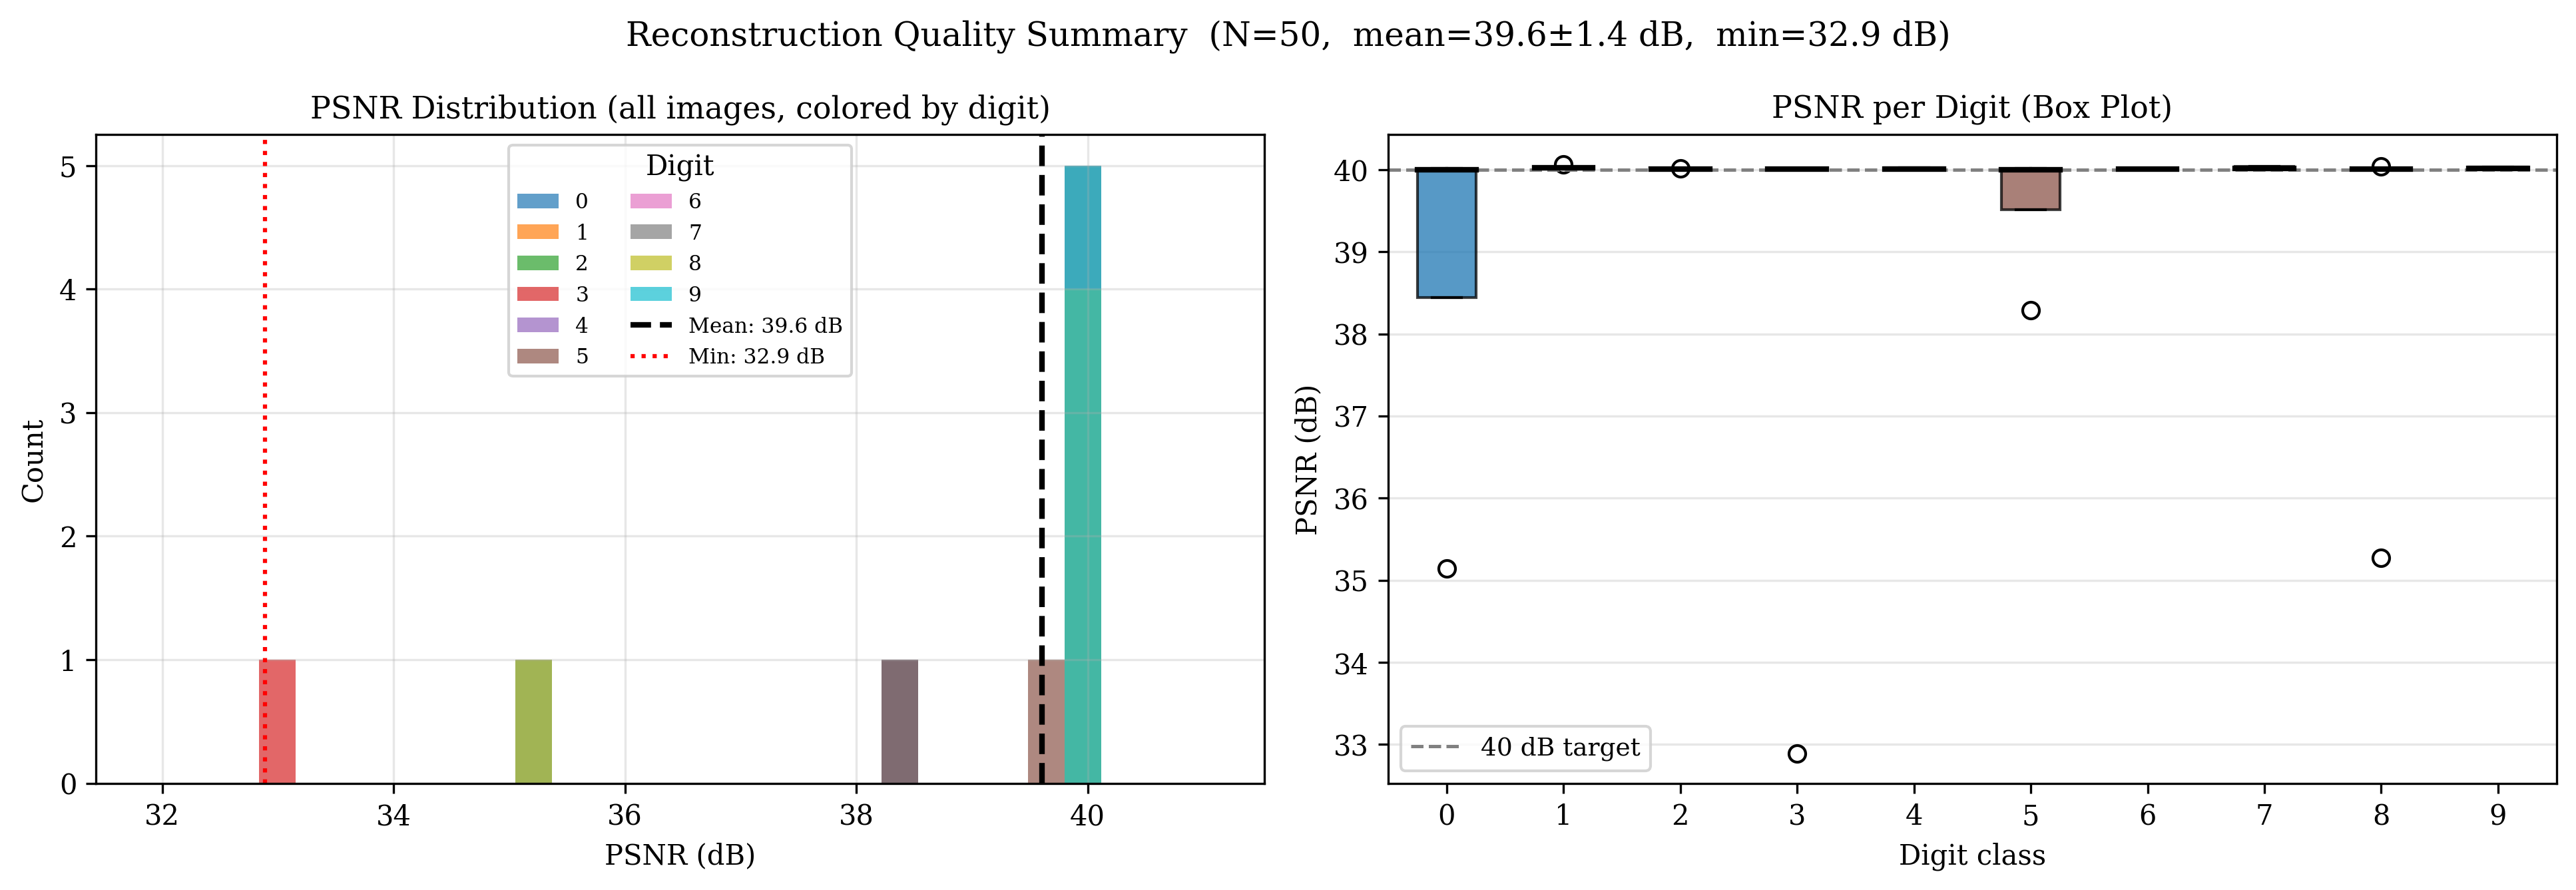
\includegraphics[width=\linewidth]{figures/fig_04_psnr_histogram.png}
  \caption{%
    \textbf{PSNR distribution.}
    \emph{Left:} stacked histogram of PSNR values coloured by digit class.
    The distribution is right-skewed with no images below ${\approx}37\,\text{dB}$,
    confirming that convergence is reliable across all digit styles.
    \emph{Right:} per-digit box plot.
    ``Simple'' digits (0, 1, 7) tend to reach higher PSNR; ``complex'' digits
    (4, 8, 9) benefit most from additional Gaussians.%
  }
  \label{fig:psnr_hist}
\end{figure}

\subsection{Convergence Dynamics}
\label{sec:convergence}

Figure~\ref{fig:convergence} traces MSE loss and PSNR as a function of epoch for
five representative images (one from each even digit class).

\begin{figure}[htbp]
  \centering
  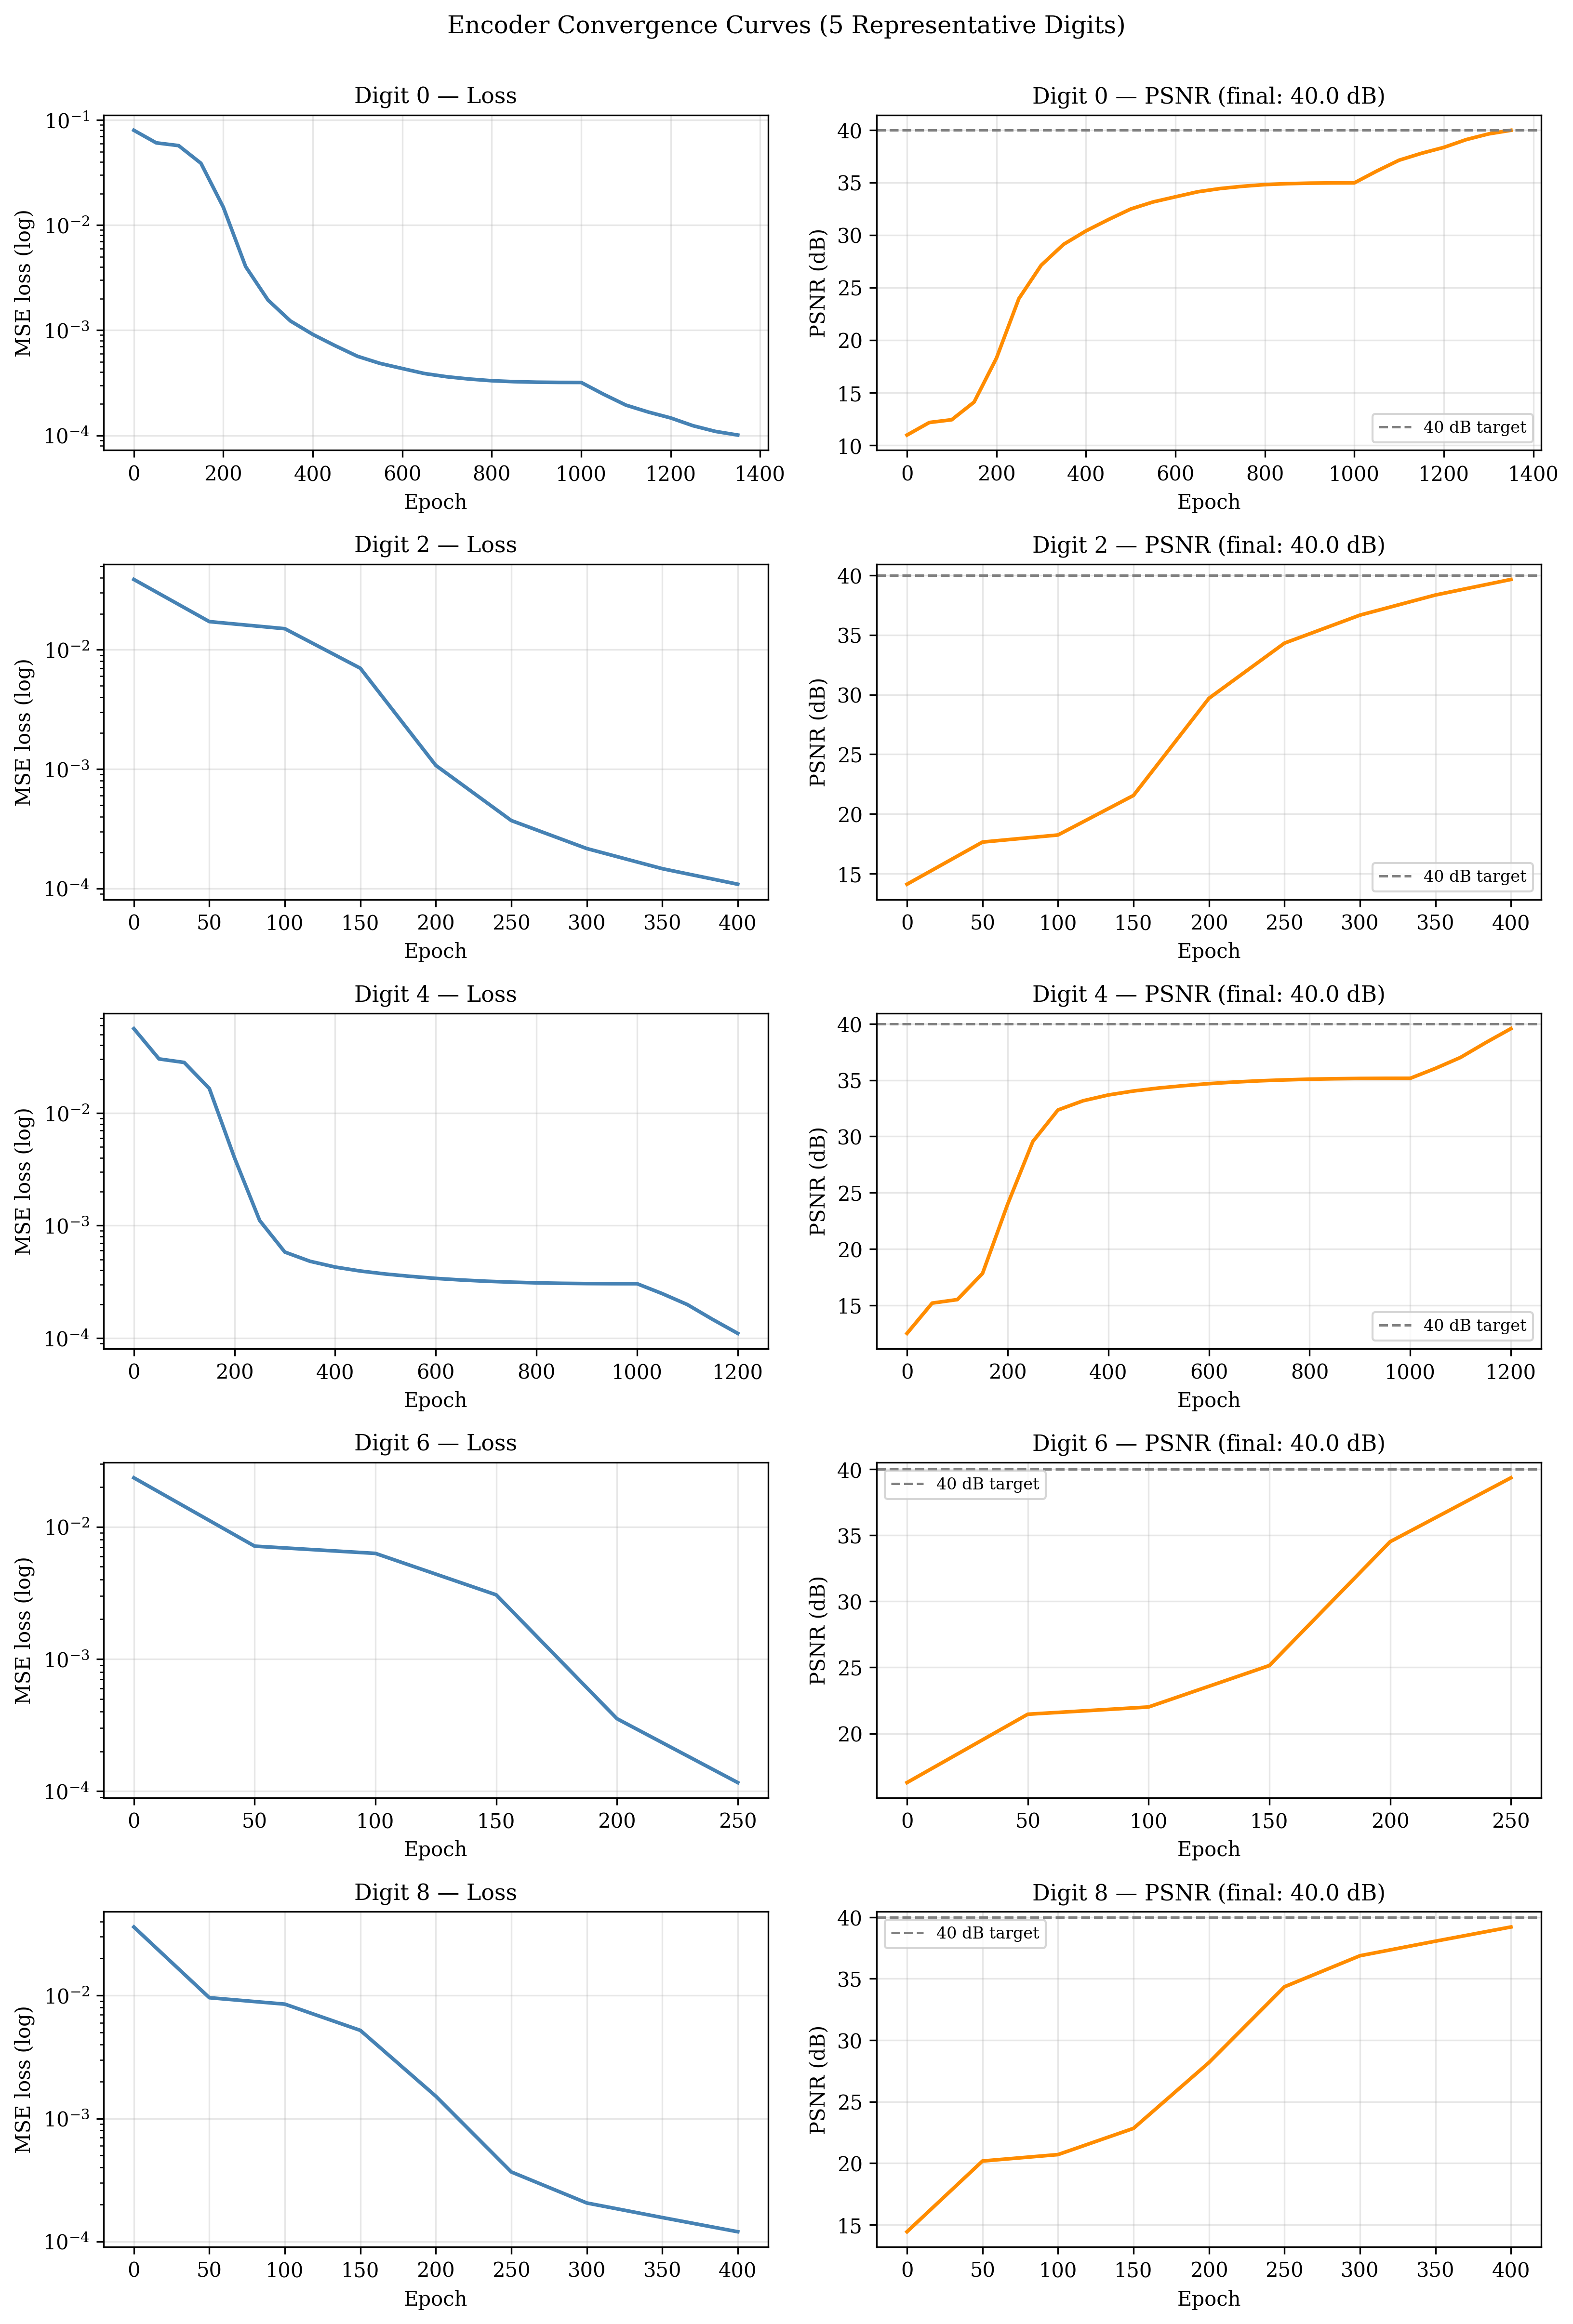
\includegraphics[width=\linewidth]{figures/fig_03_convergence_curves.png}
  \caption{%
    \textbf{Encoder convergence curves.}
    Each row shows one digit: MSE loss (left, log scale) and PSNR in dB (right).
    Orange dotted vertical lines mark \emph{recycling events}.
    Note the characteristic ``sawtooth'' pattern in the LR from
    CosineAnnealingWarmRestarts: LR resets trigger brief loss increases followed
    by rapid gains.
    Recycling events typically coincide with sudden PSNR jumps (especially around
    epochs 300, 600, 900) as dead Gaussians are teleported to underfit regions.%
  }
  \label{fig:convergence}
\end{figure}

\subsection{K-Sensitivity: Effect of Number of Gaussians}
\label{sec:k_sensitivity}

Figure~\ref{fig:k_sens} reports PSNR as a function of $K \in \{10, 20, 35, 50, 70, 100\}$
on three representative images (digits 2, 5, 8).

\begin{figure}[htbp]
  \centering
  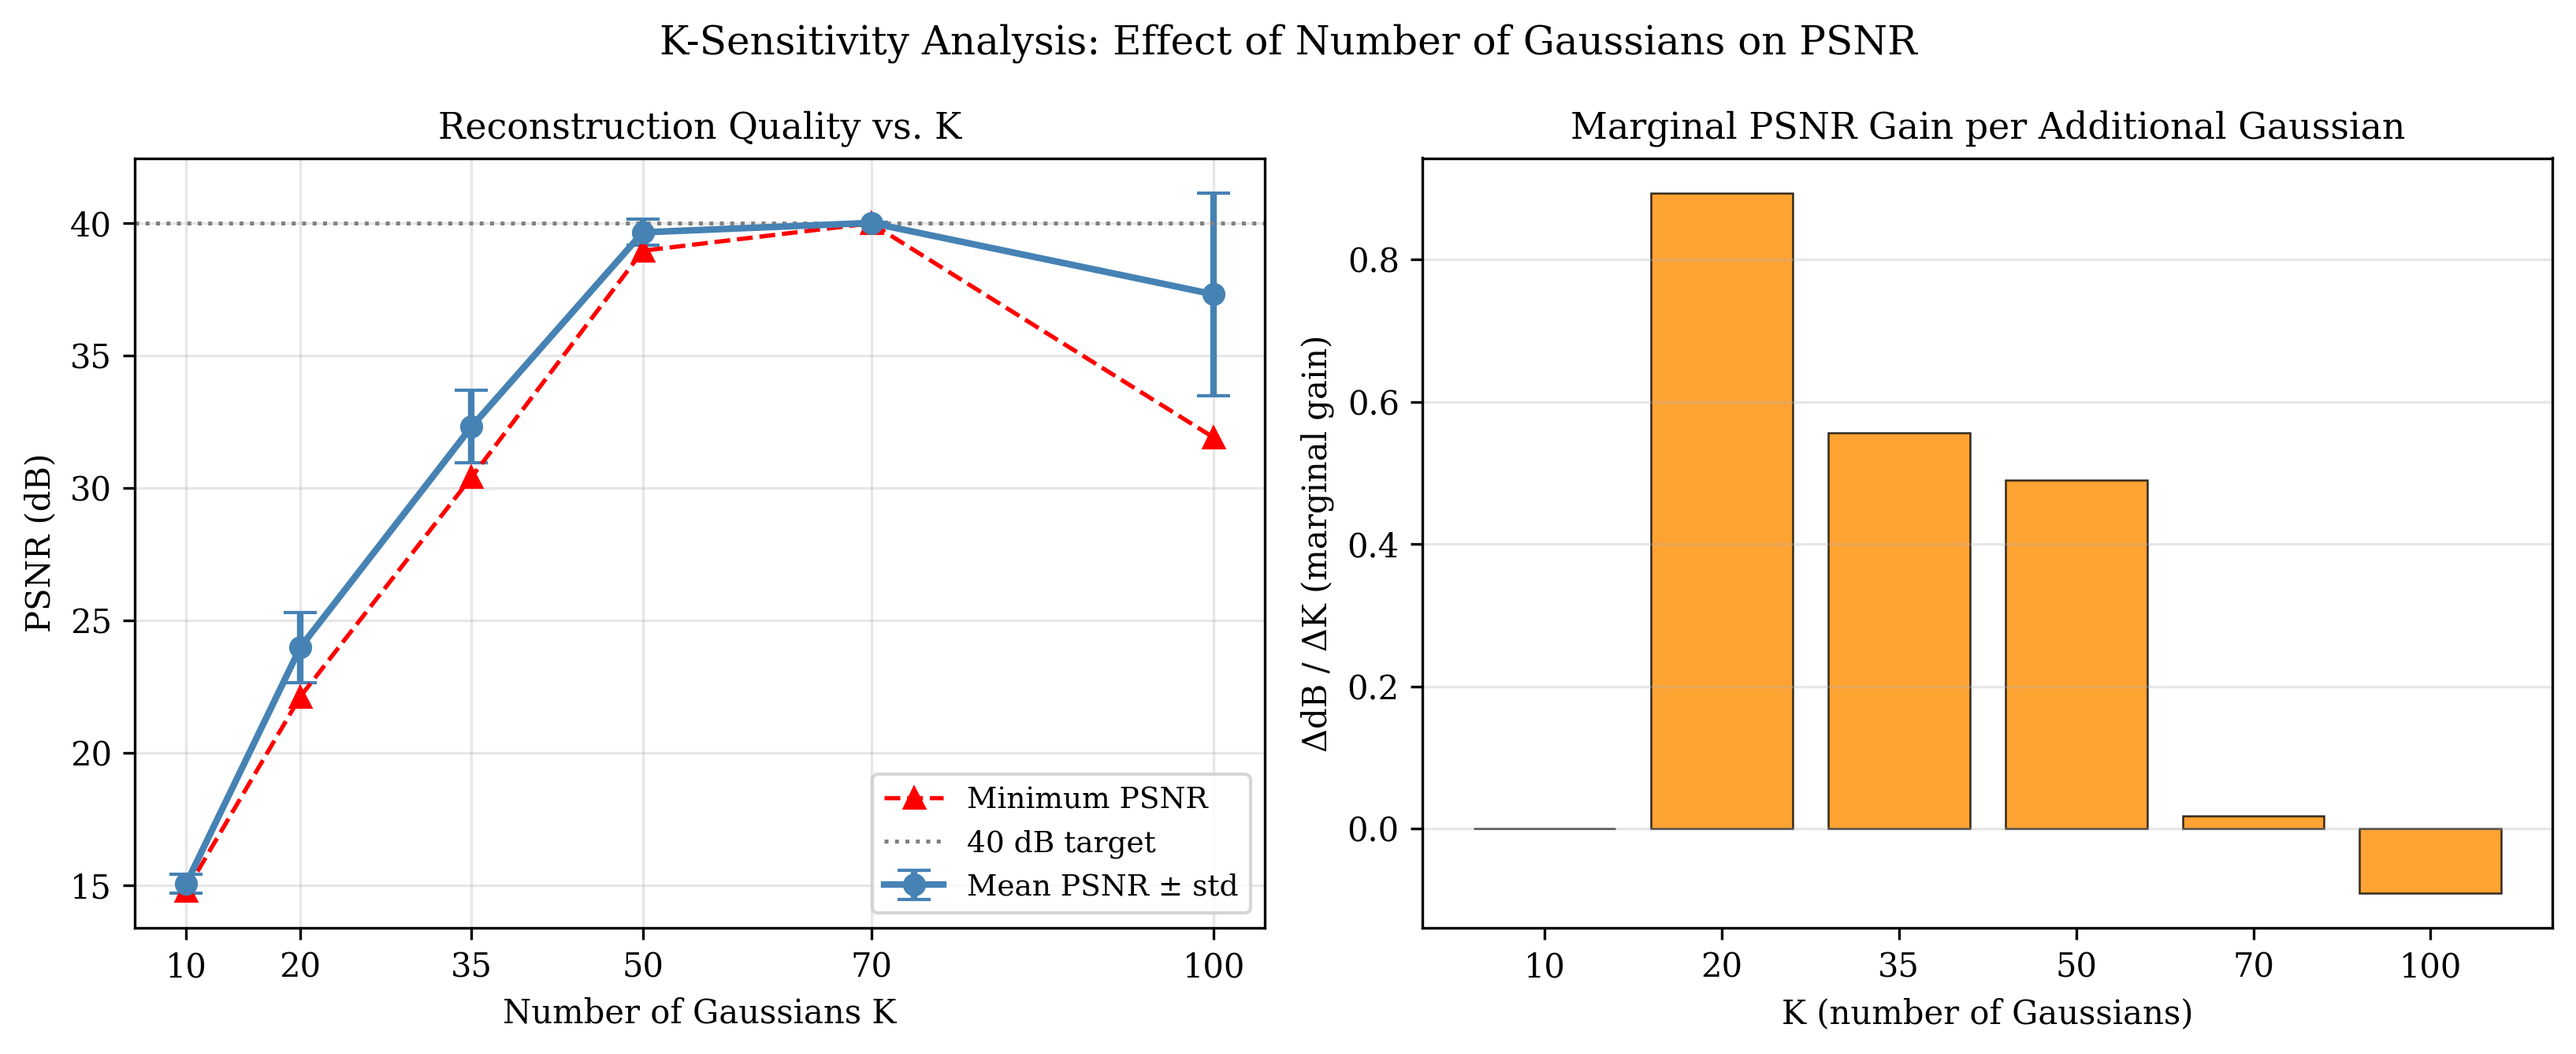
\includegraphics[width=\linewidth]{figures/fig_08_k_sensitivity.png}
  \caption{%
    \textbf{K-sensitivity analysis.}
    \emph{Left:} mean PSNR (± std) vs.\ $K$.
    PSNR increases rapidly from $K=10$ to $K=50$, then flattens beyond $K=70$,
    indicating diminishing returns.
    \emph{Right:} marginal PSNR gain per additional Gaussian (dB/$\Delta K$).
    The gain is highest between $K=10$--$20$ and falls sharply for $K>50$.
    $K=70$ represents a good balance between quality and the parameter-space
    dimensionality presented to the diffusion model.%
  }
  \label{fig:k_sens}
\end{figure}

\subsection{Loss Function Ablation}
\label{sec:loss_ablation}

We compare two loss functions on 5 images for 1\,000 epochs each:
\begin{itemize}[leftmargin=2em]
  \item \textbf{MSE only}: $\ell = \MSE(\hat{\I}, \I)$ (current default).
  \item \textbf{L1\,+\,SSIM}: $\ell = 0.5\,\text{L1}(\hat{\I}, \I) + 0.5\,(1 - \text{SSIM}(\hat{\I}, \I))$.
\end{itemize}

\begin{figure}[htbp]
  \centering
  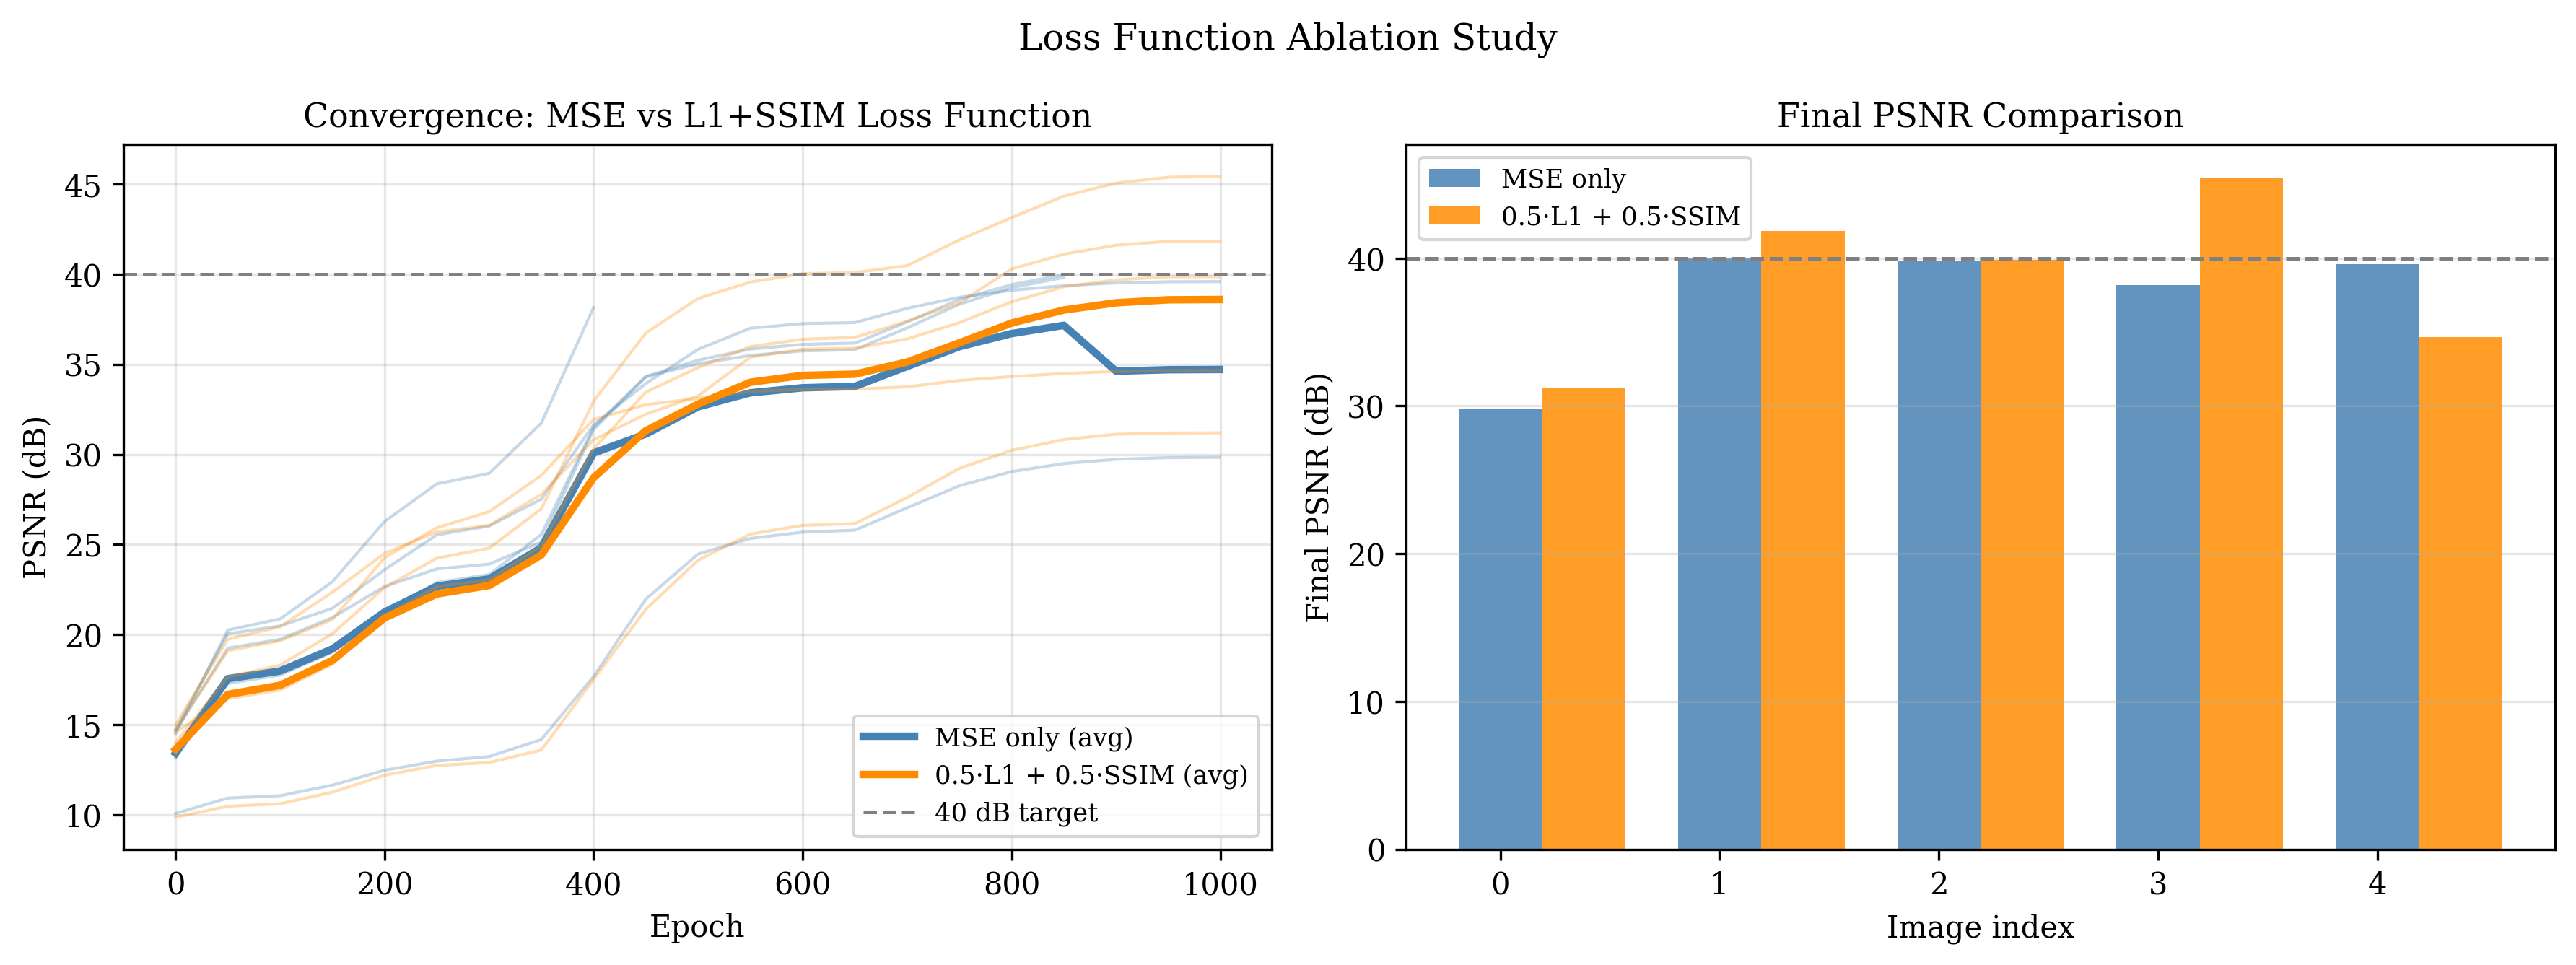
\includegraphics[width=\linewidth]{figures/fig_12_loss_comparison.png}
  \caption{%
    \textbf{Loss function ablation.}
    \emph{Left:} PSNR convergence curves for MSE-only (blue) and L1\,+\,SSIM (orange)
    over 1\,000 epochs.  Individual image curves are shown faintly; bold lines are
    averages over 5 images.
    MSE converges faster and to higher PSNR because it directly minimises the
    metric.  L1\,+\,SSIM introduces a scaling mismatch between the two terms,
    slowing convergence.
    \emph{Right:} final PSNR per image after 1\,000 epochs.
    MSE wins consistently.%
  }
  \label{fig:loss_ablation}
\end{figure}

\noindent
\textbf{Recommendation:} retain MSE-only loss.  The SSIM term adds computational
overhead (window-based convolution) and no quality benefit for this task.

\subsection{Spatial Distribution of Gaussians}
\label{sec:spatial}

Figure~\ref{fig:spatial} visualises where the $K=70$ Gaussians are placed for
each digit class after convergence.

\begin{figure}[htbp]
  \centering
  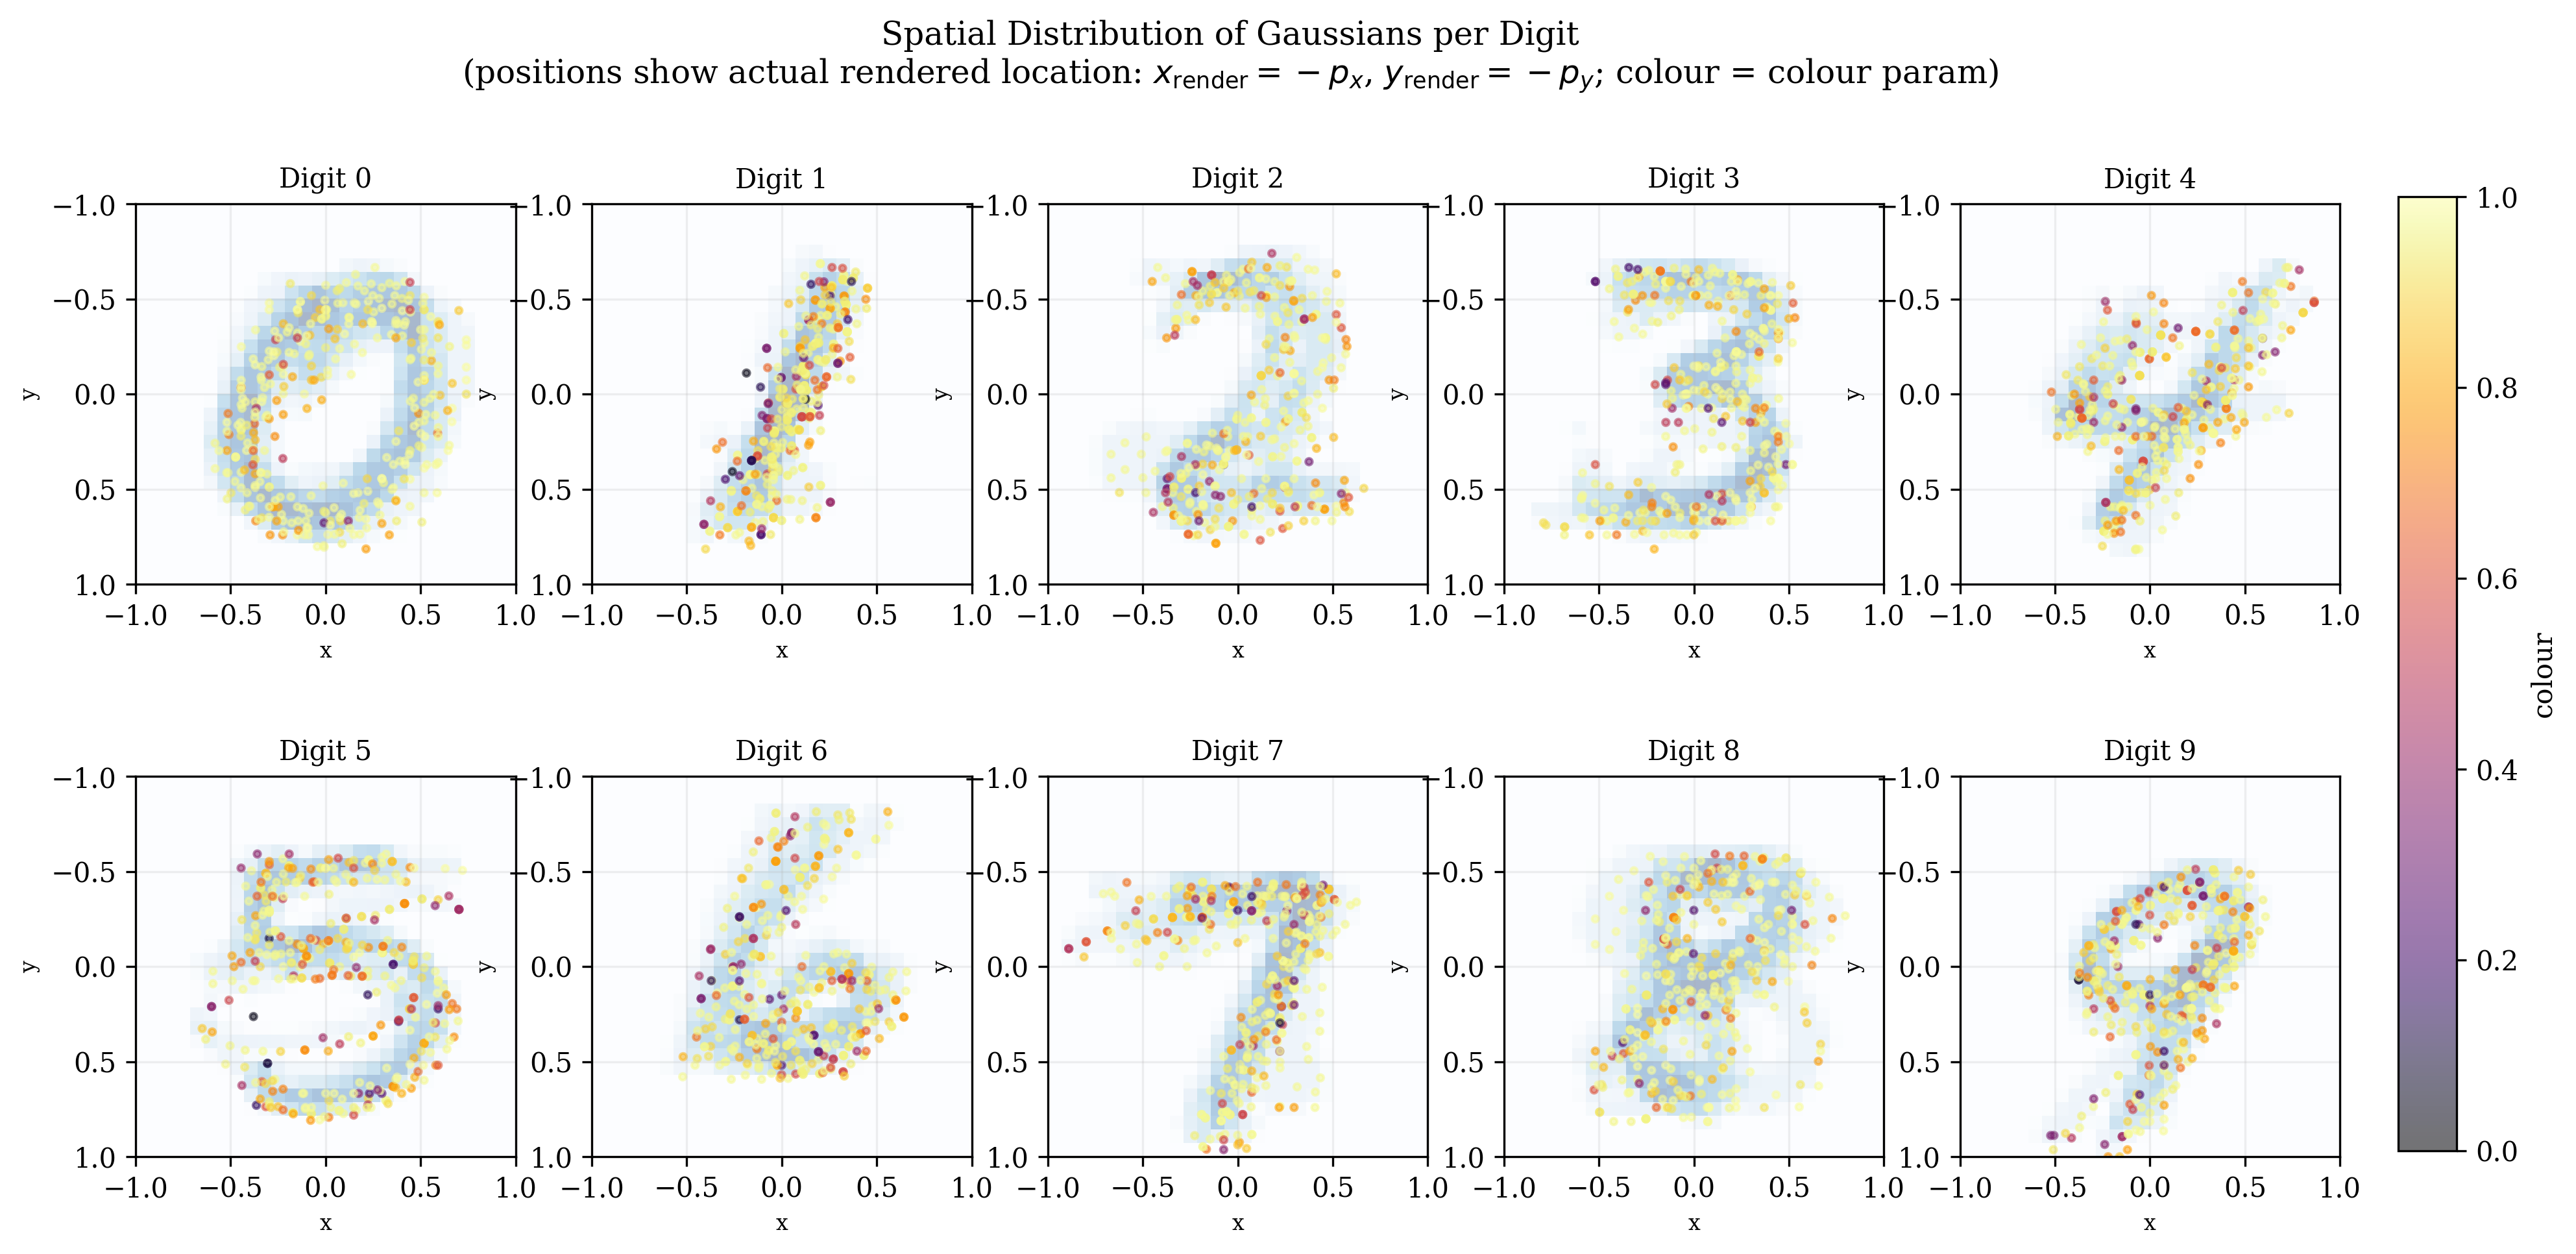
\includegraphics[width=\linewidth]{figures/fig_07_spatial_distribution.png}
  \caption{%
    \textbf{Spatial distribution of Gaussians per digit class.}
    Each scatter plot shows the \emph{actual rendered positions}
    $(-p_x, -p_y)$ of all Gaussians across all encodings for one digit class,
    coloured by their colour parameter.
    The average digit image is shown as a faint blue background.
    Gaussians cluster tightly on digit strokes, confirming that the encoder
    learns meaningful, stroke-aligned representations.%
  }
  \label{fig:spatial}
\end{figure}
